%%

% \documentclass[manuscript,anonymous,review]{acmart}
\documentclass[manuscript,screen,review]{acmart}

\usepackage{here} % [H]とするとその場所に配置されるらしい

\long\def\comment#1{}

%%
%% \BibTeX command to typeset BibTeX logo in the docs
\AtBeginDocument{%
  \providecommand\BibTeX{{%
    \normalfont B\kern-0.5em{\scshape i\kern-0.25em b}\kern-0.8em\TeX}}}

%% Rights management information.  This information is sent to you
%% when you complete the rights form.  These commands have SAMPLE
%% values in them; it is your responsibility as an author to replace
%% the commands and values with those provided to you when you
%% complete the rights form.
\setcopyright{acmcopyright}
\copyrightyear{2020}
\acmYear{2020}
\acmDOI{10.1145/1122445.1122456}

%% These commands are for a PROCEEDINGS abstract or paper.
\acmConference[Woodstock '18]{Woodstock '18: ACM Symposium on Neural
  Gaze Detection}{June 03--05, 2018}{Woodstock, NY}
\acmBooktitle{Woodstock '18: ACM Symposium on Neural Gaze Detection,
  June 03--05, 2018, Woodstock, NY}
\acmPrice{15.00}
\acmISBN{978-1-4503-XXXX-X/18/06}


%%
%% Submission ID.
%% Use this when submitting an article to a sponsored event. You'll
%% receive a unique submission ID from the organizers
%% of the event, and this ID should be used as the parameter to this command.
%%\acmSubmissionID{123-A56-BU3}

%%
%% The majority of ACM publications use numbered citations and
%% references.  The command \citestyle{authoryear} switches to the
%% "author year" style.
%%
%% If you are preparing content for an event
%% sponsored by ACM SIGGRAPH, you must use the "author year" style of
%% citations and references.
%% Uncommenting
%% the next command will enable that style.
%%\citestyle{acmauthoryear}

%%
%% end of the preamble, start of the body of the document source.
\begin{document}

%%
%% The "title" command has an optional parameter,
%% allowing the author to define a "short title" to be used in page headers.
\title{Beyond query expansion - expanding documents for fluid keyword search}

%%
%% The "author" command and its associated commands are used to define
%% the authors and their affiliations.
%% Of note is the shared affiliation of the first two authors, and the
%% "authornote" and "authornotemark" commands
%% used to denote shared contribution to the research.
\author{Toshiyuki Masui}
\email{masui@pitecan.com}
\orcid{1234-5678-9012}
\affiliation{%
  \institution{Keio University}
  \streetaddress{1234 Endo}
  \city{Fujisawa}
  \state{Kanagawa}
  \country{Japan}
  \postcode{43017-6221}
}

%%
%% By default, the full list of authors will be used in the page
%% headers. Often, this list is too long, and will overlap
%% other information printed in the page headers. This command allows
%% the author to define a more concise list
%% of authors' names for this purpose.
\renewcommand{\shortauthors}{Toshiyuki Masui}

%%
%% The abstract is a short summary of the work to be presented in the
%% article.
\begin{abstract}
  Although intelligent text search algorithms are widely available
  these days, documents are still hard to find in many cases. It is
  usually hard to find useful information in help systems and manual
  pages, even when required information exists in the documents.

  Searches fail mainly because of the ``vocabulary problem,'' where users
  cannot find the right search keyword. When a user wants to
  ``remove a file,''and there is a manual entry or ``deleting a file,'' users may
  not be able to know how to remove a file until he finds the right
  keyword ``delete'' for the search.
  To solve the problem, various \textit{query expansion}
  techniques are widely used on the Web. When a user
  types ``remove'' in the search box, the system automatically expands the
  keyword and suggests using ``remove/delete'' instead. Query expansion
  works effectively for simple cases, but it does not work well when the
  concept in the users' mind is very different from the text in the
  manual document. For example, if a user wants to ``clean up the
  desktop,'' he cannot find an appropriate manual entry that only
  describes how to ``delete icons'' or ``align icons'' on the desktop.

  We propose a new approach \textit{document expansion} for finding
  help documents and manual entries. We provide flexible explanations
  for each document using regular expression patterns. For the above
  example, we give an expression like \texttt{(delete|remove) (a file|data)}
  and use the expanded text like \texttt{delete a file}, \texttt{remove data} for
  keyword search. Also, a pattern like \texttt{(delete|remove) \#{file}} is
  expanded to \texttt{delete Makefile}, \texttt{delete search.c}, etc. depending on
  the existing files, so that a user can enter \texttt{del ma} to get
  \texttt{delete Makefile} and immediately execute it.

  We have been using this document expansion technique called
  ExpandSearch for several years, and the system is working on various
  commercial Web services. In this paper, we describe the idea and
  implementation of ExpandHelp and show how it works in the wild.
\end{abstract}

% 異なる言語でも大丈夫
% Translation paradigm


%%
%% The code below is generated by the tool at http://dl.acm.org/ccs.cfm.
%% Please copy and paste the code instead of the example below.
%%
\begin{CCSXML}
<ccs2012>
 <concept>
  <concept_id>10010520.10010553.10010562</concept_id>
  <concept_desc>Computer systems organization~Embedded systems</concept_desc>
  <concept_significance>500</concept_significance>
 </concept>
 <concept>
  <concept_id>10010520.10010575.10010755</concept_id>
  <concept_desc>Computer systems organization~Redundancy</concept_desc>
  <concept_significance>300</concept_significance>
 </concept>
 <concept>
  <concept_id>10010520.10010553.10010554</concept_id>
  <concept_desc>Computer systems organization~Robotics</concept_desc>
  <concept_significance>100</concept_significance>
 </concept>
 <concept>
  <concept_id>10003033.10003083.10003095</concept_id>
  <concept_desc>Networks~Network reliability</concept_desc>
  <concept_significance>100</concept_significance>
 </concept>
</ccs2012>
\end{CCSXML}

\ccsdesc[500]{Computer systems organization~Embedded systems}
\ccsdesc[300]{Computer systems organization~Redundancy}
\ccsdesc{Computer systems organization~Robotics}
\ccsdesc[100]{Networks~Network reliability}

%%
%% Keywords. The author(s) should pick words that accurately describe
%% the work being presented. Separate the keywords with commas.
\keywords{text search, help systems, query expansion}


%%
%% This command processes the author and affiliation and title
%% information and builds the first part of the formatted document.
\maketitle

\section{Introduction}

People are frequently searching information using keywords on Google
and other systems, but keyword search is still not an easy task,
because it is fundamentally difficulto to find appropriate information
that does not contain the keyword given by the user.

% Webでもパソコンでも情報検索はキーワード検索が主流だが、キーワード検索は昔も今も難しい
% 根本的に、[[本文に含まれていない文字列の検索が難しい]]からである

The help system of MacOS (Catalina v10.15.5) does not tell a user how to remove a file.

\begin{figure}[H]
  \centering
  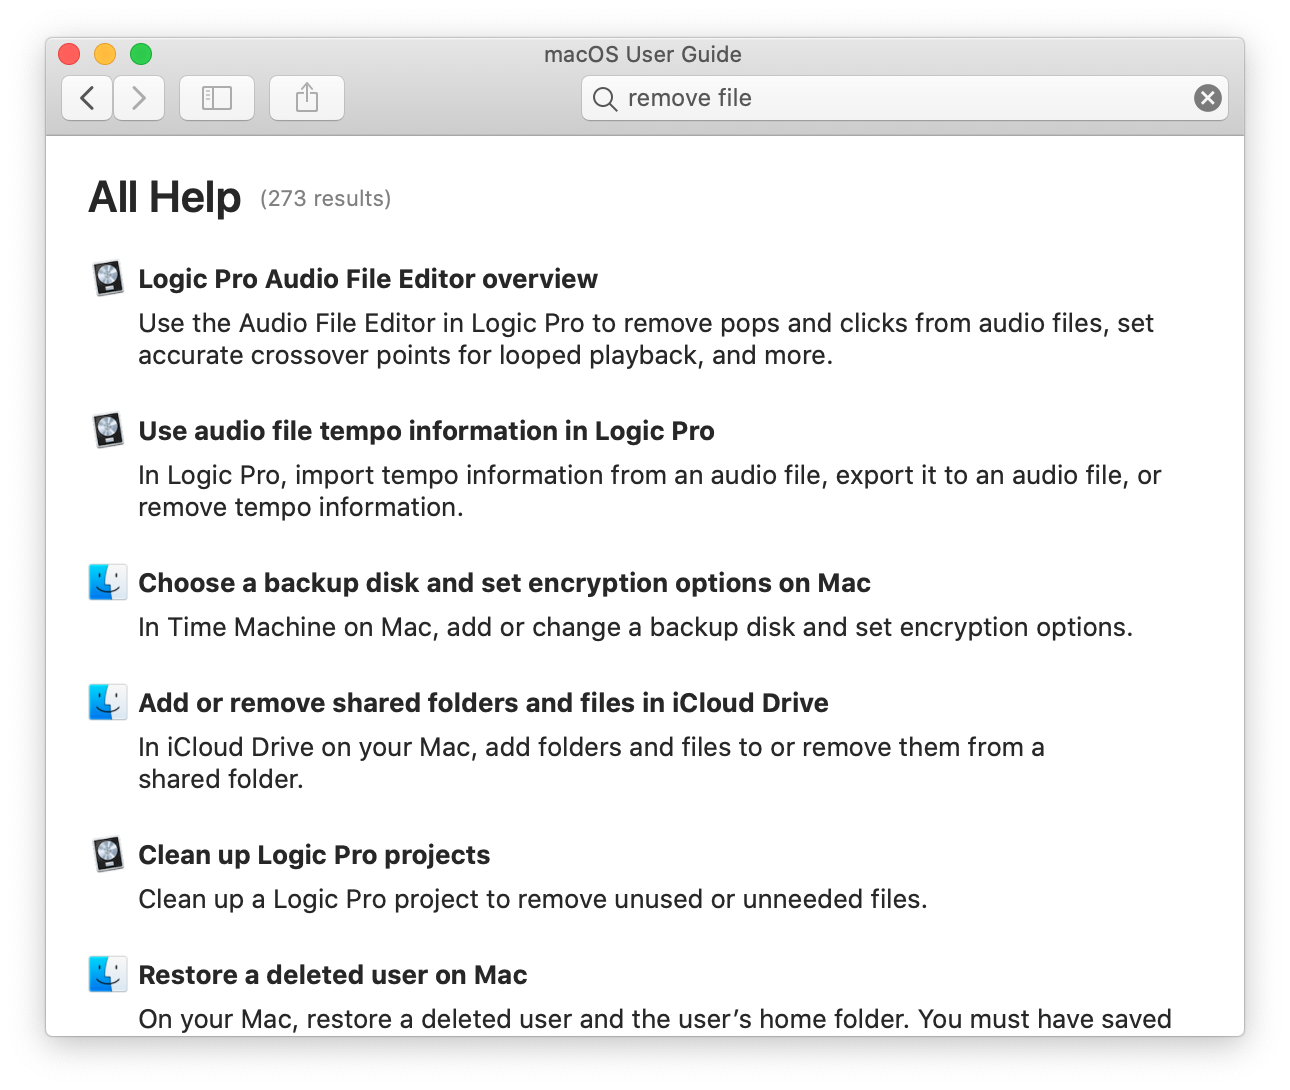
\includegraphics[width=10cm,bb=0 0 1290 1090]{figures/eaa80e41ddc3d3620fae133007274573.png}
  \caption{Asking the help application how to remove a file.}
  \Description{Mac Mac}
\end{figure}

Using the same help application, 
a user can find how to set the system clock of the computer,
but the user has to know that
``setting the clock'' and ``changing date'' means the same thing.

\begin{figure}[H]
  \centering
  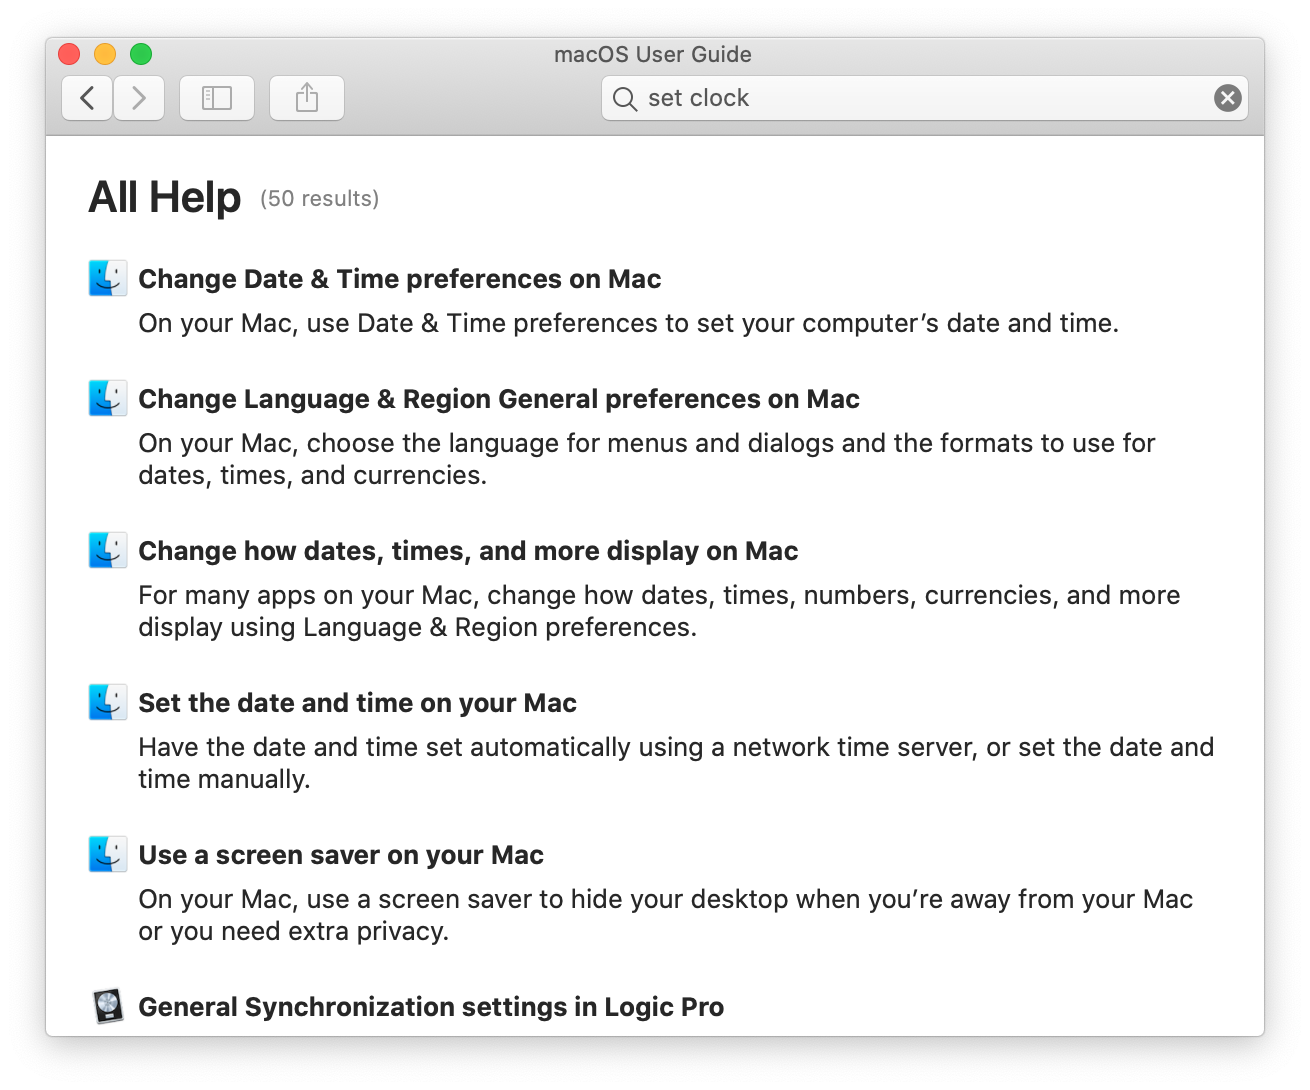
\includegraphics[width=10cm,bb=0 0 1310 1090]{figures/0cd679128d8f69eb2a8a966d6466a8a4.png}
  \caption{Mac}
  \Description{Mac Mac}
\end{figure}

We can get this kind of information fairly easily using search systems on Internet,
so many people prefer getting information using search engines rather than
using help systems provided by manufacturers.

We can find information on Google because there are tremendous information
that describe how to ``remove a file'' on Mac.
If there are documens that contain ``remove'', ``file'', and ``Mac'',
finding such documents are not easy.

That seems to be the main reason why people are satisfied with search engines on the net
for finding popular? information.

% For example we can find how to XXXX by using YYYY, because somebody on the net has written an article on XXXX using the keyword YYYY.

% Googleとかで意外とみつかる気がするのは、Web上のメジャーな情報は
% いろんな人がいろんな言葉で情報をアップしてるからだろう (出典)
% 機能を検索したとき、トップに出るのはメーカーのサイトではない
% 情報が無いからではなく、キーワードがマッチしないからだと思われる

On the other hand,
finding a less popular information is rather difficult,
because not enough document related to the topic is found on the net.

If there is only one document on the net
that describes the \texttt{console} feature of a minor system \texttt{xxxxx},
people cannot find the document using a similar keyword \texttt{dashboard}
since the document does not contain the word \texttt{dashboard}.

% メジャーじゃないシステムや特殊な状況のヘルプなどの場合、文書もユーザも少ないから苦労する
% キーワードが少しでも違うとみつからない
% 開発者の用語とユーザの用語が違うことの違いの問題がさらにひどい

% e.g. メジャーじゃないxxxxxシステムのyyyyy機能
%   Google Chrome Extensionのconsoleとかみつからない (dashboardだとみつかる)
% 	(他の例も)

FAQs provided by service providers are not usually considered useful
because the terms used by the people on the service are usually
different from the word that user can think of.

% いわゆるFAQは大抵不十分(出典)
%   特殊なサービスの特殊な機能について書かれてることが多いからだろう
%   メジャーなサービスであっても、ググって本家FAQが出てくることなど無い
%    誰かが言い替えたものがヒットするのが普通 (出典)

Even finding the users' old documents can be sometimes difficult,
because people might use different keywords for the same
thing. He might try to find a file on "ZZZ" and fail, because he used
the term "WWW" before.

% 自分のメモですら後でみつけられなくて困ることも多い
%  微妙に利用単語が違うとみつからない
%  良いファイル名をつけたつもりでも後から検索できないことがある

Various techniques have been proposed to solve this vocabulary problem.
But not very successful.

Finding documents are even more difficult when
the user's mother language is different from the language used in the document.
When a user wants to find how to ``delete a file'' but the
manual of the system is written in French,
he has to \textbf{translate} the term ``delete'' and ``file''
before the search.
Non-English speakers are always having trouble
translating the word in their brain into English words
before searching on the net.


% 母語が違うときはさらに大変である
% 頭の中の単語を英語に変換する必要がある
% 常にTranslationや言い替えが必要だといっていいだろう
% (いったん文書がみつかれば、それを理解することはできるが、そもそもみつけるのが難しいのである)
% クエリや検索技術を工夫して解決しようとする方法が多い
% 原文はいじれないから
%  いろんな言い回しで検索する研究は大昔からある

\subsection{Query Expansion}

The vocabulary problem and the translation problem can be solved
if the search system have a thesaurus and a translation dictionary.

For example, 
if the system knows that removing a file and deleting a file is the same,
the system can try to find something using the keyword ``delete'',
even when the user specified the keyword ``remove''.

This kind of technique is called \textit{Query expansion}, and simple query
expansion is possible if proper dictionary is provided.


% クエリに工夫する方法
%    シソーラス的検索の一般化
%    検索対象の本文は変わらないから不十分
%    クエリだけ拡張してもしょうがない
%    本文に固有名詞的なものが少ない場合はみつけにくい
%    e.g. 「良い論文を書く方法」「査読を通す方法」「インパクトある論文を書く方法」
%     「レビュワーを説得する技術」 vs 「良い論文を書く方法」
% ユーザが指定するあらゆるキーワードを拡張するのは不可能である
% John F. Kennedy
% 
% 翻訳してから検索するのも一種のQUery Expansionである
% 日本語を入力すると英語のWikipediaがみつかることもある => これは違う原理

Query expansion is effective when simple substitution of keywords are satisfactory enough.
Using 'delete' in addition to 'remove' works...

However, it does not work for finding a document for vague topics.
For example, if you want to find a document that describes ``how to write a good paper'',
you will have little chance finding a document related to the topic.
Maybe it would be better to use keywords like ``how to persuade reviewers''.
However, expanding a phrase like ``write a good paper'' to ``persude reviewers'' is impossible,
unless the expander knows the contents.

%  別の言い替え文書(Tipsとか逆引き辞典)を用意
%   便利だがメジャーなものに限られる
%   もと文書と全然違うところで作り直しは大変すぎるが、逆引き本は売れている
%   hands-on と言うのだろうか?
%    ちょっと違う
%    handbook かな?
%    firsthand

Similarly, 
when we want to find a library function of a programming language, query expansion does not work.
For example, when we want to write a poker game program and
want to select five cards from the deck, what library should we use?
you want to selet randomly two items from an array in Ruby,
you can use the \texttt{sample()} method.
However, ``randomly selecting items'' and \texttt{sample} are so different, it is very hard for users to
find the method unless the manual contains words like ``randomly select''.

% 「配列からランダムに要素をふたつ取得」 = `a.sample(2)`
%    `sample`という単語はなかなか出てこないのではないか
%    pick upとかselectとかchooseとか言ってしまいそう

It is even more difficult if the user wants to find information that is not easily described with keywords.
When a user wants to know what the icons on the Mac desktop mean, he might want to to 
search by saying "What is the symbol with three curved lines

\includegraphics[width=6mm,bb=0 0 225 225]{figures/fb2349ca17df1876178857566e7c68ef.png} % wifi icon
on my computer display?
(folding fan, two black 90-degree arcs above a black circcle)

%  特殊な言葉が使われていない場合は検索が難しい
%   「Macの画面の上の方の宇宙船みたいな記号」では駄目
%    「メニューバーの音声アイコン」だとみつかるかもしれないが
%  他の言語の場合でも同じである
% [[原文を拡張する感じにして、簡潔なインタフェースを用意して任意のキーワードを使えるのが良い]]

There should be better way to make everything more searchable by casual computer users.

\section{Solutions}

% [[解決策]]
%  [[解決策1:]] 展開ヘルプで徹底的に拡張/曖昧検索
%   [[検索対象側で、いろんなクエリに対応できるような工夫をしておく]]
%   あらゆるクエリにマッチするように、いろんな表現を用意しておく
%    Query をExpandするわけではなく、あらゆるQueryに対応できるように[[本文をExpandする]]
%    本文になければ、いくらQueryをExpandしてもみつからないから
%    クエリパタンで`(dashboard|console)` などと指定するのではなく、[[本文に両方書いておく]]
%    RegExpによる展開とAsearchによる曖昧検索
%   いろんな表現を用意しておけばいろんな表現で検索できるのはあたりまえだが、用意する手間は減らせる
%  [[解決策2:]] ユーザが勝手に検索対象をExpandする
%   逆引き辞典式
%   既存のキーワード検索インタフェースをユーザが拡張する
%   自分で登録 (scrapbox, 拡張機能)
%    `console`でも検索できるようにする
%   自分のデータには記述するし、他人のデータにも記述する
%  これらを[[ExpandSearch]]と呼ぶ
%   フツーの検索システムの上に皮をかぶせる形で実装する

To solve the vocabulary problem and the translation problem,
we propose the combination of three techniques described below.

\begin{enumerate}
  
\item \textbf{Using ExpandSearch}
  
  The main idea for solving the problem is 
  providing \textbf{regular expressions} (REs)
  for  each document so that a wide variety of user queries can match one of the
  strings expanded from the REs.
  
  When we want to provide a manual that describes how to delete a file, 
  we provide a RE like \verb*(delete|remove) (a file|data)*
  and generate all the text that match this RE.
  In this case, we can epand this RE into
  \verb|delete a file|,
  \verb|delete data|,
  \verb|remove a file|, and
  \verb|remove data|.
  and use all these strings for the search.
  Users can find this document by using fleible query like
  \verb|delete file| or
  \verb|remove data|.
  We can add descriptions in other languages, like \verb*(ファイル|データ)を(消す|(消去|削除)する)*
  A user can use a phrase like ``ファイルを消去する'' to find the manual page.

\item \textbf{Approximate pattern matching}

  People make spelling errors all the time, and approximate pattern matching algorithm
  works quite effectively for almost all search activities.
  Using the ExpandHelp algorithm, all the expressions are expanded in advance,
  so simple approximate pattern matching algorithms can be applied for the search.
  For example, a query like ``del dta'' can be used

\item \textbf{Document expansion by users}

  As we have shown before, one of the big reasons why we fail to find a document is that
  the user's search keyword does not exist in the document.
  Providing entries for ExpandSearch can solve the problem, but
  
  If the author of the document does not provide the data, it would be nice if
  other users can add the ExpandHelp entries.
  This strategy is very similar to writing a hands-on document for an existing document,
  but adding ExpandHelp entries is much easier than authoring  a document from scratch.

\end{enumerate}

\section{Examples}

\subsection{Helpfeel}

We have been applying ExpahdSearch for various customer support services on existing Web services.
The help system based on ExpandSearch is called \textit{Helpfeel}, and

Helpfeel is a FAQ engine that supports users who do not have enough vocabulary for the Web services they want to use.

% ここでどこかのサポートシステムを示す

Figure xxx shows an example Helpfeel page that supports finding FAQs
for PayPay Free market run by Yahoo! Japan.
We provide the description on the Scrapbox wiki service,


% https://paypayfleamarket.yahoo.co.jp/help/

\begin{figure}[H]
  \centering
  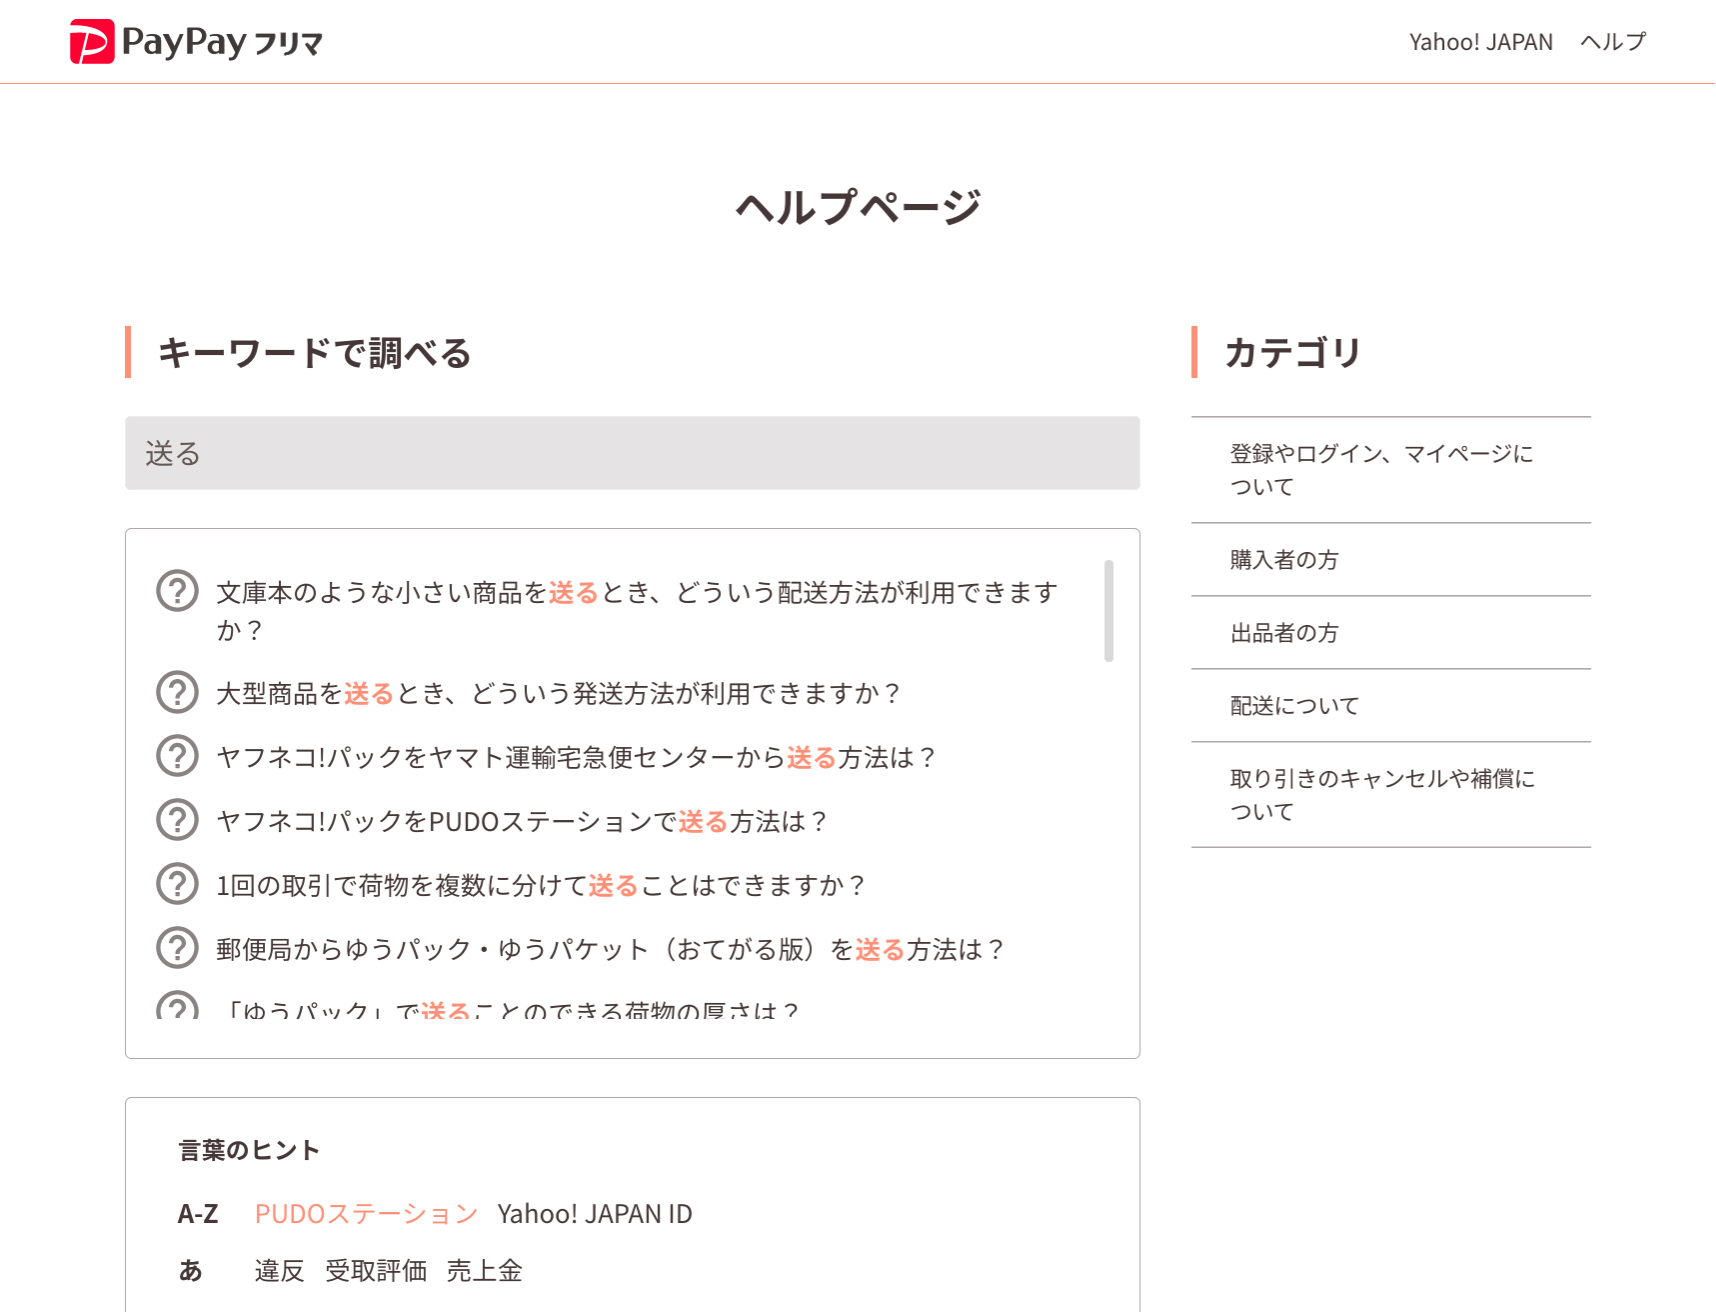
\includegraphics[width=10cm,bb=0 0 1716 1312]{figures/3d964512606a5e25646104a738ab104e.png}
  \caption{PayPay Freemarket}
  \Description{PayPay}
\end{figure}

\subsection{HelpLine}

Some Unix command line tools have many options and features, and difficult to understand in many cases.
Many programmers are recently using the git version control system, but the concept of git is difficult, and
the command line options are extremely complicated.
The total number of git manuals on unix is .....

We created the GitHelp system using ExpandHelp, so that git users can easily
remember command options and use it without perfectly remembering the git commands.

\subsection{OmniHelp}

OmniHelp is an implementation of ExpandHelp that runs on Chrome browser.
The URL window on Chrome is called omnibox, 

\begin{verbatim}
[[ExpandSearchの実例]]
 まず実例を紹介する。実装はあとで。[[評価実験にもなっている。]]
[[実例1]] ExpandHelpの実際の利用
 ScrapboxというWiki上にいろんな表現を用意しておく
 Helpfeel
  PayPayフリマなどですごく効率があがった
 実際これによりヘルプ問い合わせは劇的に減る (出典: Helpfeel)
[[実例2]] 検索インタフェースの融合
 マイHelpfeel
 検索をひとつの方法に統合する
  検索方法が複数だと面倒臭い
   ググって出なければ逆引き辞典を検索する、みたいなのは面倒
  同じ検索インタフェースでいろんなところを探すほうが簡単である
  どこにメモしたか忘れて困ることがなくなる
 自分のデータが増えていく状況のグラフを書ける!

[[実例3]]
 gitのヘルプ - コマンドラインで動くもの
  パラメタを指定して実行につなげることすらできる
\end{verbatim}

\section{Implementation}

\begin{verbatim}
[[実装]]
 ExpandHelpのアルゴリズム
  正規表現の拡張とパラメタ代入
 HelpLineの実装
  omniboxを利用するとか
\end{verbatim}

\section{Discussions}

\begin{verbatim}
    検索システムを選んでから検索キーワードを入力するのに慣れてしまっている
  この必要がないことを知ると驚きがある
 検索されやすいように工夫するとか馬鹿げてると
思うかもしれないか、ググって出なきゃ無いのと同じだということを考えると、
ある程度工夫することは意味があるし、自分が後でさがすときにも役に立つわけである
  ゲームのように記述を増やす工夫もできるかもしれない
  タイトルに迷ったら両方書くみたいな
 どこにある情報でもひとつのインタフェースでみつかるのは強烈に嬉しい

[[説得ポイント]]
 ExpandHelp
  自分が入力したキーワードが検索結果に出現する嬉しさ
 検索方法の統合
 ヘルプシステムの実績

[[関連システム / 参考文献]]
 普通の[https://en.wikipedia.org/wiki/Query_expansion クエリ拡張]
 Relevance Feedback
  検索パタンを増やすことに効果があるといえる
 [https://scrapbox.io/UIPedia/George_Furnas:_The_vocabulary_problem_in_human-system_communication Vocabulary problem]
 [文芸的プログラミング]
  ExpandHelp記述は文芸的プログラミングの一種だと思えばいい
  冗長な感じで書くといい
 [/Rubytips] の実例

日本語を入力すると英語のWikipediaがみつかることもある
 これはたぶん原文を翻訳したものを検索対象にしている
 これもDocument Expansionといえる

\end{verbatim}

\end{document}


% \endinput

